\chapter{Diskussion}

\section{Oscillometrisk fikseret-ratio}
Den oscillometriske fikseret-ratio metode er brugt i hvid udstrækning til non-invasive målinger af det systoliske og diastoliske blodtryk. Det er derfor ikke unormalt at apparatet beskrevet i denne rapport under afsnit \ref{Fikseret-ratio}, anvender fikseret-ratio fastsat ud fra empirisk data. Flere studier har også vist at denne metode har en høj nøjagtighed.\fixme{Theory of the Oscillometric Maximum and the Systolic and Diastolic Detection Ratios} Problemet med denne rigide fortolkning at det systoliske og diastoliske blodtryk altid befinder sig samme procentsats fra middel arterie trykke opstår ved individernes forskellighed.

Jiankun et al\fixme{Error Mechanisms of the Oscillometric Fixed-Ratio BloodPressure Measurement Method} opstiller en matematisk model for den oscillometriske metode medregnet arterie eftergivenheden og undersøger ud fra dette hvilke faktorer, som påvirker den fikserede-ratio og hvor stor en afvigelse, fra den sande værdi dette giver. Resultaterne af denne gennemgang er teoretiske afvigelser på op til 58 mmHg ved svær arterie stivhed. Efter som at stive arterier ofte er til stede ved  arteriosklerose er apopleksi patienter (også beskrevet i afsnit \ref{chap:Baggrund}) særlig udsatte for fejlmålinger med fikseret-ratio metoden. Den korte forklaring på dette problem er ændringer af manchet oscillotionernes kurve brede. Kurven som dannes af peak ampletuderne af oscillotionerne (se figur \ref{fig:OscillometriskMetode}) ændre karakter ved ændring af arterie stivheden. Dette illustreres bedst ved at afbillede data med normaliseret manchettryk oscillotioner over manchettrykket på arterier forskellig eftergivenhed. 

\begin{minipage}[t]{0.5\textwidth}
På figur \ref{fig:ErrorMechanismOfFixedRatio} er fejl mekanismen ved fikseret-ratio bestemt systolisk tryk (SP) og diastolisk tryl (DP) illustreret. Peak ampletuderne er normaliseret, hvilket tydeliggør ændringerne i kurve bredden, når arterie eftergivenheden ændres. Ved normale arterievægge passer de empiriske ratio værdier godt, men efter som arteriet afviger fra det normale stiger fejl estimationen af SP og DP i takt med afvigelsen af eftergivenheden. Hvis er stiverer en normalt resulterer det i en overestimation af det systoliske tryk og en underestimation af det diastoliske tryk. Overestimationen finder sted fordi den konstante ratio for det systoliske tryk (SP/MAP) nu befinder sig på et tidligere tidspunkt i tid, hvor manchet trykket er højere og derfor overestimerers SP. På samme måde som systolisk tryk overestimeres, underestimeres det diastoliske tryk fordi den konstante ratio for det diastolisk tryk (SP/MAP) nu befinder sig på et senere tidspunkt i tid, hvor manchettrykket er laverer. Det samme scenarie gør sig gældende bare modsat, for en blodtryksmåling på arterier med en højere eftergivenhed end normalt. Ændringer i arterievæggens eftergivenhed påvirker ikke estimationen af MAP, som altid befinder sig med de største oscillotioner i manchetten.

Anvendelse af oscillometrisk fikseret-ratio metoden, til at måle blodtryk på patienter med apopleksi kan være problematisk på grund arterie stivheden, som giver anledning til fejl estimationer på op til 58 mmHg. Det bør derfor overvejes om andre metoder til at estimerer det sys- og diastoliske tryk skal anvendes i stedet, for at sikre en højere nøjagtighed af blodtryksmålingerne.

Overestimationen af det systoliske blodtryk optræder ikke som fejlkilde ved konditioneringen, da her blot ønskes en total okklution af arterierne. Overestimationen giver ikke anledning til et for lavt afklemningstryk, som tillader blod til den afklemte ekstremitet. Fejlkonditionering på grund af blodtryksmålingen opstår kun ved underestimering af SYS.
\end{minipage}
\begin{minipage}[t]{0.5\textwidth}
	\begin{figure}[H]
		\centering
		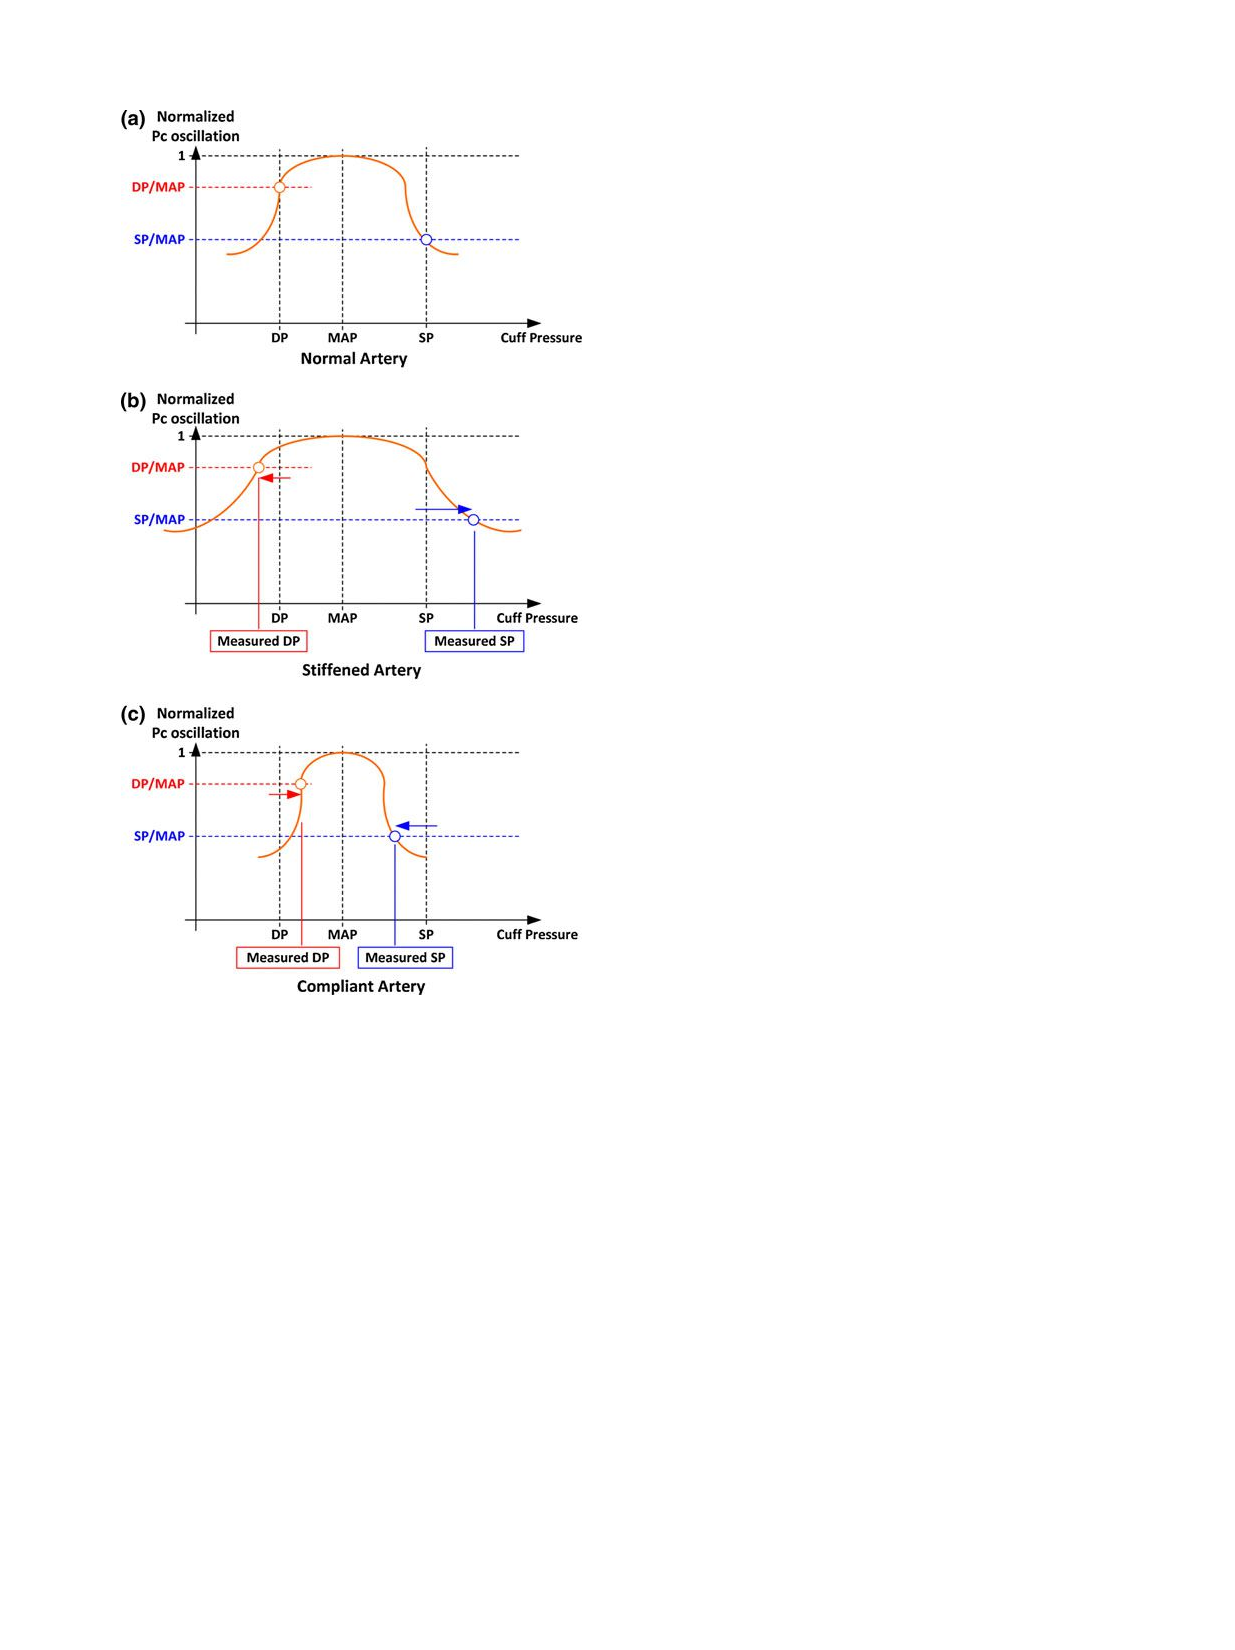
\includegraphics[width=1\textwidth]{billeder/ErrorFixed-Ratio.pdf}
		\caption{Fejl mekanismen i fixed-ratio metoden ved ændringer af arterie stivheden. Pc er manchet tryk. DP er det diastoliske tryk og SP er det systoliske tryk}\label{fig:ErrorMechanismOfFixedRatio}
	\end{figure}
	\fixme{billede Ref: Error Mechanisms of the Oscillometric Fixed-Ratio BloodPressure Measurement Method}
\end{minipage}

\section{Medicinsk godkendelse} \label{title:medGodkendelse}
Hvis konditioneringsapparatet er medicinsk udstyr, skal der opfyldes en lang række krav, for at apparatet må anvendes på patienter. I dette afsnit udledes hvilke krav produktet skal opfylde, for at kunne anvendes i klinisk forsøg og til hjemmebehandling (hjemmebehandling er beskrevet i afsnit \ref{title:Hjemmebehandling})

Konditioneringsapparatet skal i følge derektivet "93/42/EEC" Artikel 1, 2.a medicinsk godkendes fordi følgende er opfyldt.

\begin{quote}
	"medicinsk udstyr: ethvert instrument, apparat, udstyr, software,
	materiale eller anden genstand anvendt alene eller i kombination,
	herunder software, som af fabrikanten er beregnet til specifik anvendelse
	til diagnostiske og/eller terapeutiske formål, og som hører med
	til korrekt brug heraf, og som af fabrikanten er beregnet til anvendelse
	på mennesker med henblik på:
	\begin{itemize}
		\item diagnosticering, forebyggelse, overvågning, behandling eller
		lindring af sygdomme
		\item diagnosticering, overvågning, behandling, lindring af eller
		kompensation for skader eller handicap
		\item undersøgelse, udskiftning eller ændring af anatomien eller en
		fysiologisk proces
		\item svangerskabsforebyggelse
	\end{itemize}
	
	og hvis forventede hovedvirkning i eller på det menneskelige
	legeme ikke fremkaldes ad farmakologisk, immunologisk eller metabolisk
	vej, men hvis virkning kan understøttes ad denne vej" \fixme{Kilde til derektivet 93/42/EEC}
\end{quote}

Konditioneringsapparatet opfylder første punkt fordi den skal forebygge celledød i penumbra. Ydermere opfyldes punkt to også, fordi konditioneringensapparatet måler blodtrykket af patienten og dermed hjælper til diagnosticering af patienten.

Konditioneringsapparatet skal som beskrevet i baggrundsafsnittet \ref{title:studieprotokold} anvendes til et klinisk forsøg. Særlige lave krav, er gældende for medicinsk udstyr, hvor der blandt andet kun kræves de væsentlige krav.

I "BILLAG VIII: Erklæring vedrørende anordninger til særlige formål" 2.2 står der blandt andet at dokumentationen skal indeholde følgende:

\begin{quote}
	"en bekræftelse på, at den pågældende anordning er i overensstemmelse
	med de væsentlige krav undtagen for så vidt angår de aspekter, der er
	omfattet af afprøvningen, samt på at der med hensyn til disse aspekter
	er truffet alle nødvendige forholdsregler for at beskytte patientens
	helbred og sikkerhed"
\end{quote}

De væsentlige krav inderholder i det store og hele risikohåndtering af det medicinske apparat. Langt

Noter: CE godkendelse og anvendelse af ikke godkend blodtryksmåler til forskningsprojekt, med medicinsk personale til stede under hele brugen. Hjemme brug.

\section{Pulsoximetri}
Under resultat afsnittet \ref{title:pulsOxi} er der beskrevet en test, som bruger pulsoximeter for at tjekket kredsløbets status på armen under RIC behandling. Der blev kun foretaget én af sådan en test og den blev foretaget på person som er sund og rask. Derfor er testen ikke et gyldigt grundlag for at eksludere pulsoximetri som. Men teorien bag pulsoximeteri, som beskrives i projektafgrænsnings afsnittet (\ref{title:sikkerhedskontrol}), sætter tydelig begrænsninger for brugen af pulsoximetri til dette formål og testen underbygger kun denne påstand. 



